\chapter{Preliminaries}
%\pagestyle{fancy}
%\doublespacing

%%%%%%%%%%%%%%%%%%%%%%%%%%%%%%%%
%In this chapter, we recall the necessary background, terminology and facts about Coxeter systems and their associated Hecke algebras and Temperley--Lieb algebras as shown in \cite{Green1999} and \cite{Losonczy2000}. 

%%%%%%%%%%%%%%%%%%%%%%5

\section{Introduction}
This thesis is organized as follows. After necessary background material on Coxeter systems is presented in Section~\ref{sec:coxsyst}, we introduce the class of fully commutative elements in Section~\ref{sec:FC}. Then, in Section~\ref{Aheap} and Section~\ref{sec:Dheaps}, we discuss a visual representation for elements of Coxeter systems, called heaps. We then recall requisite terminology and facts about Hecke algebras in Section~\ref{hecke} and Temperley--Lieb algebras in Section~\ref{sec:TL}. In Chapter~\ref{ch:diag}, we establish our notation and introduce all of the terminology required to define an associative diagram algebra, $\DTL(D_n)$, that is a faithful diagrammatic representation of the Temperley--Lieb algebra of type $D$, $\TL(D_n)$. Next, in Section~\ref{sec:loopfree}, we construct a faithful diagrammatic representation, $\LFD(D_n)$, of a particular quotient of the Temperley--Lieb algebra, $\PFTL(D_n)$, that we introduce in Section~\ref{sec:pairfree}. After defining cellular algebras in Section~\ref{sec:cellular}, we explicitly construct a cell datum for $\LFD(D_n)$ that is used to prove the main result (Theorem~\ref{loopfreecellular} and Corollary~\ref{pairfreecellular}), which says that $\LFD(D_n)$ and therefore $\PFTL(D_n)$ are cellular. 

%The simple diagrams, introduced in Section~\ref{sec:simple}, are diagrams that generate the basis diagrams of  In Sections~\ref{undec}--\ref{sec:simple}, . In Section~\ref{sec:admissible}, we explore the diagram algebra as 
\section{Coxeter systems}\label{sec:coxsyst}
A \emph{Coxeter system} is a pair $(W,S)$ consisting of a finite set $S$ of generating involutions and a group $W$, called a \emph{Coxeter group}, with presentation
\[
W = \langle S :(st)^{m(s, t)} = e \text{ for } m(s, t) < \infty \rangle,
\] 
where $e$ is the identity, $m(s, t) = 1$ if and only if $s=t$, and $m(s, t) = m(t, s)$.  It turns out that the elements of $S$ are distinct as group elements and that $m(s, t)$ is the order of $st$. 

Since $s$ and $t$ are elements of order 2, the relation $(st)^{m(s,t)}=e$ can be rewritten as 
\begin{equation}
\label{relation}
{\underbrace{sts \cdots }_{m(s,t)} } = {\underbrace{tst \cdots}_{m(s,t)}}
\end{equation}
 with $m(s,t)\ge 2$ factors.
If $m(s,t)=2$, then $st=ts$ is called a \emph{short braid relation} and $s$ and $t$ commute. Otherwise, if $m(s,t)\ge 3$, then relation~\ref{relation} is called a \emph{long braid relation}. Replacing $\underbrace{sts \cdots }_{m(s,t)}$ with $\underbrace{tst \cdots}_{m(s,t)}$ will be referred to as a \emph{braid move}.
\\

We can represent $(W,S)$ with a unique \emph{Coxeter graph}, $\Gamma$, having: 
\begin{enumerate}[leftmargin=0.6in]
\item vertex set $S$; 
%\item edges $\{s,t\}$ whenever $m(s,t)\ge 3$; 
%\item edges $\{s,t\}$ unlabeled whenever $m(s,t)=3$;
\item edges $\{s,t\}$ labeled with $m(s,t)$ for all $m(s,t)\ge3$.
\end{enumerate}
Since $m(s,t)\ge 3$ occurs most frequently, it is customary to leave the corresponding edge unlabeled.


If $(W,S)$ is a Coxeter system with Coxeter graph $\Gamma$, then for emphasis, we may denote the group as $W(\Gamma)$. There is a one-to-one correspondence between Coxeter systems and Coxeter graphs. Given the Coxeter graph $\Gamma$, we can uniquely reconstruct the corresponding Coxeter system. Note that generators $s$ and $t$ are not connected in the Coxeter graph if and only if $s$ and $t$ commute. In addition, the Coxeter group $W$ is said to be \emph{irreducible} if and only if the corresponding Coxeter graph is connected. If the Coxeter graph is disconnected, the connected components correspond to factors in a direct product of irreducible Coxeter groups \cite[Section 2.2]{Humphreys.J:A}.
 

\begin{example}
~
\begin{itemize}
\item[(a)~] We define $A_{n}$ to be the Coxeter graph in Figure~\ref{fig:Agraph}. Given $A_{n}$, we can construct $\(\WA, S\)$ with the generators $\left\{ s_{1},s_{2},\ldots,s_{n}\right\} $ and defining relations
\begin{align*}
s_{i}^2&=  e & \text{for all }i,\\
s_{i}s_{j}&=  s_{j}s_{i} & \text{when }\left|i-j\right|>1,\\
s_{i}s_{j}s_{i}&=  s_{j}s_{i}s_{j} & \text{when }\left|i-j\right|=1.
\end{align*}

\noindent The Coxeter group $\WA$ is isomorphic to the symmetric group $S_{n+1}$ under $s_{i}\mapsto \(i,i+1\)$. 

\item[(b)~] We define $D_{n}$ to be the Coxeter graph in Figure~\ref{fig:Dgraph}. Given $D_{n}$, we can construct $\(\WD, S\)$ with the generators $\left\{ s_{\overline{1}},s_{1},s_{2},\ldots,s_{n-1}\right\} $ and defining relations
\begin{align*}
s_{i}^2&=  e & \text{for all }i,\\
s_{i}s_{j}&=  s_{j}s_{i} & \text{when }\left|i-j\right|>1 \text{ for }i, j \in \left\{1,2,\ldots,n\right\},\\
s_{i}s_{j}s_{i}&=  s_{j}s_{i}s_{j} & \text{when }\left|i-j\right|=1 \text{ for }i, j \in \left\{1,2,\ldots,n\right\}, \\
s_{\overline{1}}s_{i}&=  s_{i}s_{\overline{1}} & \text{for all }i\in \left\{1,3,\ldots,n\right\},\\
s_{\overline{1}}s_{2}s_{\overline{1}}&=  s_{2}s_{\overline{1}}s_{2}.
\end{align*}

\noindent The Coxeter group $\WD$ is isomorphic to $S_{n}^{D}$, where $S_{n}^{D}$ is the subgroup of the group of signed permutations having an even number of sign changes, called the \emph{group of even signed permutations}. The main focus of this thesis will be the Coxeter system of type $D_n$.
\end{itemize}
\end{example}

\begin{figure}[h]
\centering
\begin{subfigure}[b]{0.4\textwidth}
\centering
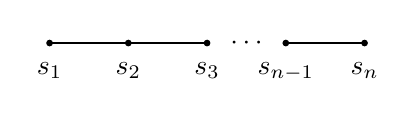
\begin{tikzpicture} \draw[fill=black] \foreach \x in {1,2,3,4,5} {(\x,10) circle (1pt)}; \draw \foreach \x in {1,2,3} {(\x,10) node[label=below:$s_{\x}$]{}};  \draw {(4,10) node[label=below:$s_{n-1}$]{}}; \draw {(5,10) node[label=below:$s_{n}$]{}}; \draw {(3.5,10) node[]{$\cdots$}}; \draw[-] (1,10) -- (2,10); \draw[-] (2,10) -- (3,10); \draw[-] (4,10) -- (5,10); \end{tikzpicture}
\caption{Type $A_{n}~\(n\ge 2\)$}
\label{fig:Agraph}
\end{subfigure}
\quad
\begin{subfigure}[b]{0.4\textwidth}
\centering
\begin{tikzpicture} \draw[fill=black] \foreach \x in {2,3,4,5} {(\x,10) circle (1pt)}; \draw \foreach \x in {2,3} {(\x,10) node[label=below:$s_{\x}$]{}}; \draw[fill=black] \foreach \x in {9.5,10.5} {(1,\x) circle (1pt)}; \draw {(1,9.5) node[label=below:$s_{\overline{1}}$]{}}; \draw {(1,10.5) node[label=above:$s_{1}$]{}}; \draw {(4,10) node[label=below:$s_{n-2}$]{}}; \draw {(5,10) node[label=below:$s_{n-1}$]{}}; \draw {(3.5,10) node[]{$\cdots$}}; \draw[-] (1,9.5) -- (2,10); \draw[-] (1,10.5) -- (2,10); \draw[-] (2,10) -- (3,10); \draw[-] (4,10) -- (5,10); \end{tikzpicture} 
\caption{Type $D_{n}~\(n\ge 4\)$}
\label{fig:Dgraph}
\end{subfigure}
\caption{Coxeter graphs corresponding to Coxeter systems of type $A_{n}$ and $D_{n}$.}
\label{fig:graphs}
\end{figure}



Given a Coxeter system $(W,S)$, a word $s_{x_1}s_{x_2}\cdots s_{x_m}$ in the free monoid on $S$ is called an \emph
{expression} for $w\in W$ if it is equal to $w$ when considered as a group element. If $m$ is minimal among all expressions for $w$, the corresponding word is called a \emph{reduced expression} for $w$. In this case, we define the \emph{length} of $w$ to be $\ell(w):=m$. Given $w \in W$, if we wish to emphasize a fixed, possibly reduced, expression for $w$, we represent it as $\w=s_{x_1}s_{x_2}\cdots s_{x_m}.$
%\]an \emph{expression} is a product of generators from $S$.  The \emph{length} of an element $w \in W$, $l(w)$, is the minimum number of generators appearing in any expression for the element $w$.  Such a minimum length expression is called a \emph{reduced expression}. Each element $w \in W$ can have several different reduced expressions that represent it.
\begin{theorem}
{\rm (Geck,~\cite[Matsumoto's Theorem]{Geck2000})} If $w \in W$, then every reduced expression for $w$ can be obtained from any other by applying a sequence of braid moves of the form 
\[
{\underbrace{sts \cdots }_{m(s,t)} } \mapsto {\underbrace{tst \cdots}_{m(s,t)}}
\]
where $s,t \in S$ and $m(s,t)\ge 2$.\qed 
\end{theorem}
It follows from Matsumoto's theorem that any two reduced expressions for $w \in W$ have the same number of generators in the expression. The \emph{support} of an element $w \in W$, denoted $\supp(w)$, is the set of all generators appearing in any reduced expression for $w$, which is well-defined by Matsumoto's Theorem. We will use $\w$ to represent a fixed expression, possibly reduced, for $w \in W$. We define a \emph{subexpression} of $\w$ to be any subsequence of $\w$.  If $x \in W(\Gamma)$ has an expression that is equal to a subexpression of $\w$, then we write $x \leq w$.  This is a well-defined partial order \cite[Chapter 5]{Humphreys.J:A} on $W(\Gamma)$ and is called the \emph{(strong) Bruhat order}. We will refer to a consecutive subexpression of $\w$ as a \emph{subword}. 

Let $w \in W$.  We define
\[
\L(w):=\{s \in S: \ell(sw) < \ell(w)\}
\]
and
\[
\R(w):=\{s\in S:\ell(ws)<\ell(w)\}.
\]

\noindent The set $\L(w)$ is called the \emph{left descent set} of $w$ and $\R(w)$ is called the \emph{right descent set}. It turns out that $s \in \L(w)$ if and only if $w$ has a reduced expression beginning with $s$ and $s \in \R(w)$ if and only if $w$ has a reduced expression ending with $s$.

\begin{example}
Let $w\in W(A_{4})$ and let $\w =s_{1}s_{2}s_{1}s_{4}s_{2}$ be an expression for $w$. Then
\begin{align*}
s_{1}s_{2}s_{1}s_{4}s_{2}&=  s_{2}s_{1}s_{2}s_{4}s_{2}\\
&=  s_{2}s_{1}s_{2}s_{2}s_{4} \\
&=  s_{2}s_{1}s_{4}. 
\end{align*}
This shows that $\w$ is not reduced. However, it turns out that $s_{2}s_{1}s_{4}$ is a reduced expression for $w$ and hence $l(w)=3$. Note that $\L(w)=\{s_2,s_4\},\R(w)=\{s_1,s_4\}$, and $s_{1}s_{4}$ is a subword of $\w$.
\end{example}

 



%%%%%%%%%%%%%%%%%%%%%%

\section{Fully commutative}\label{sec:FC}

Let $(W,S)$ be a Coxeter system of type $\Gamma$ and let $w \in W$. Following Stembridge~\cite{Stembridge1996}, we define a relation $\sim$ on the set of reduced expressions for $w$. Let $\w_1$ and $\w_2$ be two reduced expressions for $w$. We define $\w_1 \sim \w_2$ if we can obtain $\w_1$ from $\w_1$ by applying a single commutation move of the form $st\mapsto ts$, where $m(s,t)=2$. Now, define the equivalence relation $\approx$ by taking the reflexive transitive closure of $\sim$. Each equivalence class under $\approx$ is called a \emph{commutation class}. If $w$ has a single commutation class, then we say that $w$ is \emph{fully commutative}. That is, $w$ is fully commutative if any two reduced expressions for $w$ can be transformed into each other by a sequence of short braid relations. We denote the set of all fully commutative elements of $W$ by $\FC(\Gamma)$ where $\Gamma$ is the corresponding Coxeter graph to $(W,S)$. The following theorem shows that we never have an opportunity to apply a long braid relation when $w$ is fully commutative.

\begin{theorem}\label{stem}
{\rm(Stembridge, \cite{Stembridge1996})} An element $w\in W$ is fully commutative if and only if no reduced expression for $w$ contains ${\underbrace{sts \cdots }_{m(s,t)} }$ as a subword for $m(s,t)\ge3$.
\textcolor{black}{\qed}
\end{theorem}

\begin{remark}\label{subwords}
The elements of $FC(D_n)$ are precisely those whose reduced expressions avoid consecutive subwords of the type $s_{i}s_{j}s_{i}$ when $s_{i}$ and $s_{j}$ are connected in the Coxeter graph of type $D_n$
\end{remark}

\begin{example}
Figure~\ref{fig:commclasses} depicts all possible reduced expressions of $w$ and the relationships among them via commutations and long braid moves. It is clear by inspection that there are two commutation classes for $w$ represented by the two boxes, hence $w$ is not fully commutative.

\begin{figure}[h]
\centering
\begin{tikzpicture}
\draw (0,0) -- (4,0) -- (4,-5) -- (0,-5) -- (0,0);
\node at (2,-1) {$s_3s_1s_2s_3s_4$};
\tikzset{>=latex}
\draw [green, <->,>=stealth] (2,-1.5) to (2,-3.5) node[scale=0.85, left] at (2,-2.5) {$s_1s_3=s_3s_1$};
\node at (2,-4) {$s_1s_3s_2s_3s_4$};
\draw [red, <->,>=stealth] (4.5,-4) to (6.5,-4) node[scale=0.85, below] at (5.5,-4) {$s_3s_2s_3=s_2s_3s_2$};
\draw (7,0) -- (11,0) -- (11,-5) -- (7,-5) -- (7,0);
\node at (9,-1) {$s_1s_2s_3s_4s_2$};
\tikzset{>=latex}
\draw [cyan, <->,>=stealth] (9,-1.5) to (9,-3.5) node[scale=0.85, right] at (9,-2.5) {$s_2s_4=s_4s_2$};
\node at (9,-4) {$s_1s_2s_3s_2s_4$};
\end{tikzpicture}
\caption{Commutation classes for a non-fully commutative element.}
\label{fig:commclasses}
\end{figure}

%Let $w\in W(A_{4})$ and let $\w_1 =s_{3}s_{1}s_{2}s_{3}s_{4}$ be a reduced expression for $w$. By applying the the commutation $s_3s_1=s_1s_3$, we obtain another reduced expression, $\w_2=s_1s_3s_2s_3s_4$, such that $\w_1\approx\w_2$. But, by applying the long braid relation, $s_3s_2s_3=s_2s_3s_2$, we can obtain a third reduced expression, $\w_3=s_1s_2s_3s_2s_4$ which is in a different commutation class. Then, by applying the commutation $s_2s_4=s_4s_2$ to $\w_3$, we obtain the reduced expression $\w_4=s_1s_2s_3s_4s_2$ where $\w_3\approx\w_4$. Hence, $w$ is not fully commutative since $\w$ has two commutation classes.
%\begin{center}
%\begin{tabular}{| c |} 
%\fcolorbox{green}{white}{$s_{3}s_{1}$}$s_{2}s_{3}s_{4}$\\
%$\updownarrow$ \\
%\fcolorbox{green}{white}{$s_{3}s_{1}$}$s_{2}s_{3}s_{4}$
%\end{tabular}
%\begin{tabular}{| c |} 
%\fcolorbox{green}{white}{$s_{3}s_{1}$}$s_{2}s_{3}s_{4}$\\
%$\updownarrow$ \\
%\fcolorbox{green}{white}{$s_{3}s_{1}$}$s_{2}s_{3}s_{4}$
%\end{tabular}
%\end{center}
%Therefore, the original diagram equals \\ \fcolorbox{deeppink}{white}{$d_1 d_4 d_8 d_{10}$} \fcolorbox{lightorange}{white}{$d_3 d_5 d_9$} \fcolorbox{lightskyblue}{white}{$d_2 d_4 d_6$} \fcolorbox{softplum}{white}{$d_1 d_3 d_5 d_7$}
%\fcolorbox{naugreen}{white}{$d_2 d_4 d_6 d_8$} \fcolorbox{orchid}{white}{$d_1 d_3 d_5$} \fcolorbox{brickorange}{white}{$d_2 d_4$}.
\end{example}

\begin{example}
Figure~\ref{fig:commclass} depicts all possible reduced expressions of $w$ and the relationships among them via only commutations. In this case, we see that every reduced expression for $w$ can be obtained from another via a sequence of commutation moves, and hence there is only one commutation class for $w$. Therefore $w$ is fully commutative. It is also clear that there is never an opportunity to apply a long braid relation, which agrees with Theorem~\ref{stem}.

\begin{figure}[h]
\centering
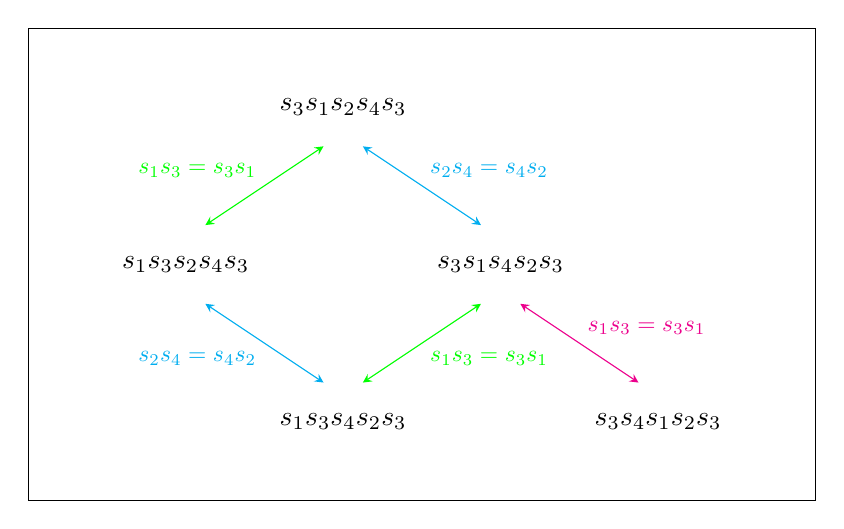
\begin{tikzpicture}
\draw (-1,0) -- (9,0) -- (9,-6) -- (-1,-6) -- (-1,0);
\node at (3,-1) {$s_3s_1s_2s_4s_3$};
\tikzset{>=latex}
\draw [green, <->,>=stealth] (2.75,-1.5) to (1.25,-2.5) node[scale=0.85, above left] at (2,-2) {$s_1s_3=s_3s_1$};
\draw [cyan, <->,>=stealth] (3.25,-1.5) to (4.75,-2.5) node[scale=0.85, above right] at (4,-2) {$s_2s_4=s_4s_2$};
\node at (1,-3) {$s_1s_3s_2s_4s_3$};
\node at (5,-3) {$s_3s_1s_4s_2s_3$};
\draw [green, <->,>=stealth] (4.75,-3.5) to (3.25,-4.5) node[scale=0.85, below right] at (4,-4) {$s_1s_3=s_3s_1$};
\draw [cyan, <->,>=stealth] (1.25,-3.5) to (2.75,-4.5) node[scale=0.85, below left] at (2,-4) {$s_2s_4=s_4s_2$};
\node at (3,-5) {$s_1s_3s_4s_2s_3$};
\draw [magenta, <->,>=stealth] (5.25,-3.5) to (6.75,-4.5) node[scale=0.85, above right] at (6,-4) {$s_1s_3=s_3s_1$};
\node at (7,-5) {$s_3s_4s_1s_2s_3$};
\end{tikzpicture}
\caption{Commutation class for a fully commutative element.}
\label{fig:commclass}
\end{figure}
%Let $w\in W(A_{4})$ and let $\w_1 =s_{3}s_{1}s_{2}s_{4}s_{3}$ be a reduced expression for $w$. By applying the the commutation $s_3s_1=s_1s_3$ to $\w_1$, we obtain another reduced expression, $\w_2=s_1s_3s_2s_4s_3$, such that $\w_1\approx\w_2$. We then can apply the commutation $s_2s_4=s_4s_2$ to $\w_2$ to obtain the reduced expression $\w_3=s_1s_3s_4s_2s_3$ where $\w_2\approx\w_3$. Then, we can apply the commutation $s_1s_3=s_3s_1$ to $\w_3$ to obtain the reduced expression $\w_4=s_3s_1s_4s_2s_3$ where $\w_3\approx\w_4$. Lastly, we can apply the commutation $s_1s_4=s_4s_1$ to $\w_4$ to obtain the reduced expression $\w_5=s_3s_4s_1s_2s_3$ where $\w_4\approx\w_5$. Hence, $w$ is fully commutative since $\w$ has a single commutation class.
\end{example}

Stembridge classified the irreducible Coxeter groups that contain a finite number of fully commutative elements, the so-called \emph{FC-finite Coxeter groups}.  While $W(D_{n})$ is a finite Coxeter group, and therefore contains a finite number of fully commutative elements, there are examples of infinite Coxeter groups that contain a finite number of fully commutative elements.  For example, Coxeter groups of type $E_n$ for $n\geq 9$ (see Figure~\ref{fig:cfcfg}) are infinite, but contain only finitely many fully commutative elements.

\begin{theorem}{\rm (Stembridge,~\cite{Stembridge1996})}
The irreducible FC-finite Coxeter groups are the Coxeter groups of type $A_{n}\left(n\ge 1\right),$ $B_{n}\left(n\ge 2\right),$ $D_{n}\left(n\ge 4\right),$ $E_{n}\left(n\ge 6\right),$ $F_{n}\left(n\ge 4\right),$ $H_{n}\left(n\ge 3\right)$ and $I_{2}\left(m\right)\left(3\le m<\infty \right)$ with corresponding Coxeter graphs shown in Figure~\ref{fig:cfcfg}. \qed
\end{theorem}


\begin{figure}[h]
\centering
\begin{tabular}{ll}
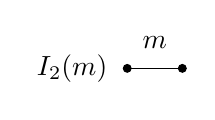
\begin{tikzpicture}[scale=.7]%I_{2}(m)
\draw[fill=black] \foreach \x in {1,2} {(\x,0) circle (2pt)};
\draw {(0,0) node{$I_{2}(m)$}
(1.5,0) node[label=above:$m$]{}
[-] (1,0) -- (2,0)};
\end{tikzpicture}
& \\
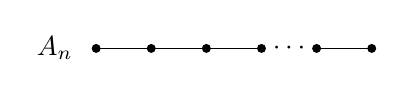
\begin{tikzpicture}[scale=.7]%A_{n}
\draw[fill=black] \foreach \x in {1,2,...,6} {(\x,10) circle (2pt)};
\draw {(.25,10) node{$A_{n}$}
(4.5,10) node{$\cdots$}
[-] (1,10) -- (4,10)
[-] (5,10) -- (6,10)}; 
\end{tikzpicture}
&
\quad  \quad \begin{tikzpicture}[scale=.7]%E_{n}
\draw[fill=black] \foreach \x in {1,2,...,6} {(\x,4.5) circle (2pt)};
\draw[fill=black] (3,5.5) circle (2pt);
\draw {(.25,4.5) node{$E_{n}$}
(4.5,4.5) node{$\cdots$}
[-] (1,4.5) -- (4,4.5)
[-] (5,4.5) -- (6,4.5)
[-] (3,4.5) -- (3,5.5)};
\end{tikzpicture}\\
\\
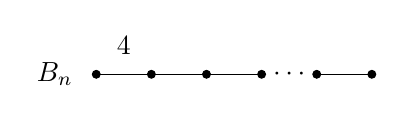
\begin{tikzpicture}[scale=.7]%B_{n}
\draw [fill=black] \foreach \x in {1,2,...,6} {(\x,8.5) circle (2pt)};
\draw {(.25,8.5) node{$B_{n}$}
(1.5,8.5) node[label=above:$4$]{}
(4.5,8.5) node{$\cdots$}
[-] (1,8.5) -- (4,8.5)
[-] (5,8.5) -- (6,8.5)}; 
\end{tikzpicture}
&
\quad  \quad \begin{tikzpicture}[scale=.7]%F_{n}
\draw[fill=black] \foreach \x in {1,2,...,6} {(\x,3) circle (2pt)};
\draw {(.25,3) node{$F_{n}$}
(2.5,3) node[label=above:$4$]{}
(4.5,3) node{$\cdots$}
[-] (1,3) -- (4,3)
[-] (5,3) -- (6,3)};
\end{tikzpicture}\\
\\
\begin{tikzpicture}[scale=.7]
\draw[fill=black] \foreach \x in {1,2,...,6} {(\x,6.5) circle (2pt)};%D_{n}
\draw[fill=black] (2,7.5) circle (2pt);
\draw {(.25,6.5) node{$D_{n}$}
(4.5,6.5) node{$\cdots$}
[-] (1,6.5) -- (4,6.5)
[-] (5,6.5) -- (6,6.5)
[-] (2,6.5) -- (2,7.5)};
\end{tikzpicture}
&
\quad  \quad 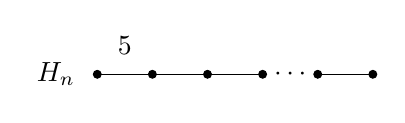
\begin{tikzpicture}[scale=.7]
\draw[fill=black] \foreach \x in {1,2,...,6} {(\x,1.5) circle (2pt)};%H_{n}
\draw {(.25,1.5) node{$H_{n}$}
(1.5,1.5) node[label=above:$5$]{}
(4.5,1.5) node{$\cdots$}
[-] (1,1.5) -- (4,1.5)
[-] (5,1.5) -- (6,1.5)}; 
\end{tikzpicture}
\end{tabular}
\caption{Coxeter graphs corresponding to the irreducible FC-finite Coxeter groups.}
\label{fig:cfcfg}
\end{figure}

%%%%%%%%%%%%%%%%%%%%%%%%%

\section{Heaps in type $A_{n}$}\label{Aheap}

Every reduced expression can be associated with a labeled partially ordered set (poset) called a heap. Heaps provide a visual representation of a reduced expression while preserving the relations among the generators. For simplicity, we will first define heaps corresponding to Coxeter groups of type $A_{n}$ and mimic the development found in \cite{Billey2007}, \cite{Ernst2010a}, and \cite{Stembridge1996}.  

Let $(W,S)$ be a Coxeter system.  Suppose $\w = s_{x_1} \cdots s_{x_k}$ is a fixed reduced expression for $w \in \WA$.  We define a partial ordering on the indices $\{1, \dots, k\}$ by the transitive closure of the relation $j \lessdot i$ if $i < j$ and $s_{x_i}$ and $s_{x_j}$ do not commute.  In particular, since $\w$ is reduced, $j \lessdot i$ if $i < j$ and $s_{x_i} = s_{x_j}$ by transitivity.  This partial order is referred to as the \emph{heap} of $\w$, where $i$ is labeled by $s_{x_i}$. Each heap corresponds to a commutation class and it follows from \cite{Stembridge1996} that $w$ is fully commutative if and only if there is a unique heap associated to $w$.

\begin{example}\label{ex:Hasse}
Let $\w=s_{2}s_{1}s_{3}s_{2}s_{4}s_{5}$ be a reduced expression for $w \in \FC(A_{5})$. We see that $\w$ is indexed by $\{1,2,3,4,5,6\}$. For example, $6 \lessdot 5$ since $5<6$ and $s_{4}$ and $s_{5}$ do not commute. The labeled Hasse diagram for the heap poset of $w$ is shown in Figure~\ref{fig:hasse}. 
\begin{figure}[h]
\centering
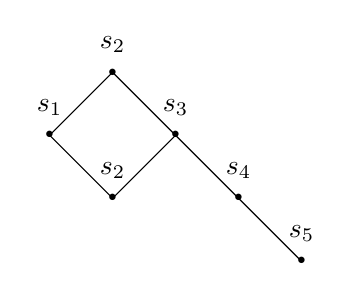
\begin{tikzpicture}[scale=0.8]
\node[scale=0.6, label=above:$s_{2}$] at (1,5.5) {$\bullet$};
\node[scale=0.6, label=above:$s_{1}$] at (0,4.5) {$\bullet$};
\node[scale=0.6, label=above:$s_{3}$] at (2,4.5) {$\bullet$};
\node[scale=0.6, label=above:$s_{2}$] at(1,3.5) {$\bullet$};
\node[scale=0.6, label=above:$s_{4}$] at(3,3.5) {$\bullet$};
\node[scale=0.6, label=above:$s_{5}$] at (4,2.5) {$\bullet$};
\draw (1,5.5)--(0,4.5)--(1,3.5)--(2,4.5)--(3,3.5)--(4,2.5);
\draw (1,5.5)--(2,4.5);
\end{tikzpicture}
\caption{Labeled Hasse diagram for the heap of a fully commutative element.}
\label{fig:hasse}
\end{figure}
\end{example}

Let $\w$ be a fixed reduced expression for $w \in W(A_{n})$.  As in \cite{Billey2007} and \cite{Ernst2010a}, we will represent a heap for $\w$ as a set of lattice points embedded in $\{1,2,\ldots,n\} \times \mathbb{N}$.  To do so, we assign coordinates (not unique) $(x,y) \in \{1,2,\ldots, n+1\} \times \mathbb{N}$ to each entry of the labeled Hasse diagram for the heap of $\w$ in such a way that:
\begin{enumerate}[leftmargin=0.6in]
\item An entry with coordinates $(x,y)$ is labeled $s_i$ (or $i$) in the heap if and only if $x = i$; 

\item If an entry with coordinates $(x,y)$ is greater than an entry with coordinates $(x',y')$ in the heap then $y > y'$.
\end{enumerate}

In the case of type $A_{n}$ and other straight line Coxeter graphs, it follows from the definition that $(x,y)$ covers $(x',y')$ in the heap if and only if $x = x' \pm 1$, $y > y'$, and there are no entries $(x'', y'')$ such that $x'' \in \{x, x'\}$ and $y'< y'' < y$.  This implies that we can completely reconstruct the edges of the Hasse diagram and the corresponding heap poset from a lattice point representation. A lattice point representation of a heap allows us to visualize potentially cumbersome arguments.  Note that entries on top of a heap correspond to generators occurring to the left  in the corresponding reduced expression.  


Let $\w$ be a reduced expression for $w \in W(A_{n})$.  We let $H(\w)$ denote a lattice representation of the heap poset in $\{1,2,\ldots,n+1\} \times \N$.  If $w$ is fully commutative, then the choice of reduced expression for $w$ is irrelevant, in which case, we will often write $H(w)$ and we will refer to $H(w)$ as the heap of $w$.  Note that if $w\in \FC(A_n)$, then entries on the top of a heap correspond to $s_i\in \L(w)$.

Given a heap, every generator will have a fixed $x$-co\-or\-di\-nate, yet the $y$-co\-or\-di\-nates may differ.  In particular, two entries labeled by the same generator will possess the same $x$-co\-or\-di\-nate but may differ by the amount of vertical space between them.

Let $\w=s_{x_1}\cdots s_{x_k}$ be a reduced expression for $w \in W(A_{n})$.  If $s_{x_i}$ and $s_{x_j}$ are adjacent generators in the Coxeter graph with $i<j$, then we must place the point labeled by $s_{x_i}$ at a level that is above the level of the point labeled by $s_{x_j}$.  Because generators that are not adjacent in the Coxeter graph do commute, points whose $x$-coordinates differ by more than one can slide past each other or land at the same level.  To emphasize the covering relations of the lattice representation we will enclose each entry of the heap in a $2\times 2$ square in such a way that if one entry covers another, the squares overlap halfway. We will also label the squares with $i$ to represent the generator $s_{i}$.

\begin{example}
Let $\w=s_1s_2s_4$ be a reduced expression for $w\in \FC(A_4)$. Figure~\ref{fig:multirep}  shows two representations for the heap of $w$. 
\begin{figure}[h]
\centering
\begin{subfigure}[b]{0.3\textwidth}
\centering
\begin{tikzpicture}[scale=0.8]
\sq{0}{7};
\node at (0.5,6.5) {$1$};
\sq{1.5}{6};
\node at (2,5.5) {$4$};
\sq{0.5}{6};
\node at (1,5.5) {$2$};
%\sq{0}{5};
%\node at (0.5,4.5) {$1$};
\end{tikzpicture}
\caption{}
\end{subfigure}
\begin{subfigure}[b]{0.3\textwidth}
\centering
\begin{tikzpicture}[scale=0.8]
\sq{0}{7};
\node at (0.5,6.5) {$1$};
\sq{1.5}{7};
\node at (2,6.5) {$4$};
\sq{0.5}{6};
\node at (1,5.5) {$2$};
\end{tikzpicture}
\caption{}
\label{canonical}
\end{subfigure}
\caption{Two possible representations for the heap of a fully commutative element.}
\label{fig:multirep}
\end{figure}
\end{example}

\begin{example}\label{multipleheaps}
Let $\w_1=s_1s_3s_2s_1$ be a reduced expression for $w\in W(A_3)$. By applying the short braid relation, $s_{1}s_{3}=s_{3}s_{1}$, we can obtain another reduced expression, $\w_2=s_3s_1s_2s_1$ which is in the same commutation class as $\w_1$, and hence has the same heap. But, by applying the long braid relation, $s_1s_2s_1=s_2s_1s_2$, we can obtain a third reduced expression $\w_3=s_3s_2s_1s_2$, which is in a different commutation class. The representations of $H(\w_1)$, $H(\w_2)$, and $H(\w_3)$ are given in Figure~\ref{fig:multiheap} where we have color-coded the blocks of the heap that correspond to the long braid relation, $s_1s_2s_1=s_2s_1s_2$.
\begin{figure}[h]
\centering
\begin{subfigure}[b]{0.3\textwidth}
\centering
\begin{tikzpicture}[scale=0.8]
\csq{0}{7};
\node at (0.5,6.5) {$1$};
\sq{1}{7};
\node at (1.5,6.5) {$3$};
\csq{0.5}{6};
\node at (1,5.5) {$2$};
\csq{0}{5};
\node at (0.5,4.5) {$1$};
\end{tikzpicture}
\caption{$H(\w_1)$ and $H(\w_2)$}
\label{commclass}
\end{subfigure}
\begin{subfigure}[b]{0.3\textwidth}
\centering
\begin{tikzpicture}[scale=0.8]
\sq{1}{7};
\node at (1.5,6.5) {$3$};
\csq{0.5}{6};
\node at (1,5.5) {$2$};
\csq{0}{5};
\node at (0.5,4.5) {$1$};
\csq{0.5}{4};
\node at (1,3.5) {$2$};
\end{tikzpicture}
\caption{$H(\w_3)$}
\label{commclasstwo}
\end{subfigure}
\caption{Two heaps for a non-fully commutative element.}
\label{fig:multiheap}
\end{figure}

%\noindent Note that $\w_1$ and $\w_2$ are in the same commutation class and therefore have the same heap as shown in Figure~\ref{commclass}, but $\w_3$ is in a different commutation class with a different heap as shown in Figure~\ref{commclasstwo}.
\end{example}
When $w$ is fully commutative, we wish to make a canonical representation of $H(w)$ by giving all entries corresponding to elements in $\L(w)$ the same vertical position and all other entries in the heap should have the highest vertical position possible (as in Figure~\ref{canonical}).

%\begin{example}\label{firstheap}
%Let $\w=s_{2}s_{1}s_{3}s_{2}s_{4}s_{5}$ as in Example \ref{ex:Hasse}.  The canonical representation for $H(w)$ is given in Figure~\ref{fig:heap}.
%\begin{figure}[h]
%\centering
%\begin{tikzpicture}[scale=0.8]
%\sq{0.5}{6};
%\node at (1,5.5) {$2$};
%\sq{0}{5};
%\node at (0.5,4.5) {$1$};
%\sq{1}{5};
%\node at (1.5,4.5) {$3$};
%\sq{0.5}{4};
%\node at(1,3.5) {$2$};
%\sq{1.5}{4};
%\node at(2,3.5) {$4$};
%\sq{2}{3};
%\node at (2.5,2.5) {$5$};
%\end{tikzpicture}
%\caption{A heap for a fully commutative element in $W(A_{5})$.}
%\label{fig:heap}
%\end{figure}
%\end{example}

% Note that since each heap corresponds to a commutation class and since $w$ in Example~\ref{multipleheaps} is not fully commutative, then there is more than one commutation class and therefore more than one heap associated to $w$. Although, if $w$ is fully commutative as in Example~\ref{firstheap}, then there is a unique heap.



Let $w \in \FC(A_n)$ have reduced expression $\w=s_{x_1}\cdots s_{x_k}$ and suppose $s_{x_i}$ and $s_{x_j}$ equal the same generator $s_m$, so that the corresponding entries have $x$-coordinate $m$ in $H(w)$.  We say that $s_{x_i}$ and $s_{x_j}$ are \emph{consecutive} if there is no other occurrence of $s_{m}$ occurring between them in $\w$.  In this case, $s_{x_i}$ and $s_{x_j}$ are consecutive in $H(w)$, as well.

Let $\w=s_{x_{1}} \cdots s_{x_{k}}$ be a reduced expression for $w \in W(A_{n})$.  We define a heap $H'$ to be a \emph{subheap} of $H(\w)$ if $H'=H(\w')$, where $\w'=s_{y_1}s_{y_2} \cdots s_{y_m}$ is a subexpression (not necessarily a subword) of $\w$.  

A subposet $Q$ of a poset $P$ is called \emph{convex} if $y \in Q$ whenever $x < y < z$ in $P$ and $x, z \in Q$.  We will refer to a subheap as a \emph{convex subheap} if the underlying subposet is convex.  

\begin{example}
Let $\w= s_{2}s_{1} s_{3}s_{2} s_{4}s_{5}$, as in Example \ref{ex:Hasse}.  Now, let $\w'=s_{2}s_{3}s_{2}$ be the subexpression of $\w$ that results from deleting all but the first, third, and fourth generators of $\w$.  Then $H(\w')$ equals the heap given in Figure~\ref{fig:subheap} and is a subheap of $H(\w)$, but is not convex since there is an entry in $H(\w)$ labeled by $s_{1}$ occurring between the two consecutive occurrences of $s_{2}$ that does not occur in $H(\w')$.  However, if we do include the entry labeled by $s_{1}$, then we obtain the heap in Figure~\ref{fig:heapheap}, which is a convex subheap of $H(\w)$. Note that if we delete the occurrence of the block labeled by $1$ in the original heap, then the heap in Figure~\ref{fig:subheap} is a convex subheap.
\end{example}

\begin{figure}[!h]
\centering
\begin{subfigure}[b]{0.3\textwidth}
\centering
\begin{tikzpicture}[scale=0.8]
\sq{0.5}{6};
\node at (1,5.5) {$2$};
\sq{1}{5};
\node at (1.5,4.5) {$3$};
\sq{0.5}{4};
\node at(1,3.5) {$2$};
\end{tikzpicture}
\caption{}
\label{fig:subheap}
\end{subfigure}
\begin{subfigure}[b]{0.3\textwidth}
\centering
\begin{tikzpicture}[scale=0.8]
\sq{0.5}{6};
\node at (1,5.5) {$2$};
\sq{0}{5};
\node at (0.5,4.5) {$1$};
\sq{1}{5};
\node at (1.5,4.5) {$3$};
\sq{0.5}{4};
\node at(1,3.5) {$2$};
\end{tikzpicture}
\caption{}
\label{fig:heapheap}
\end{subfigure}
\caption{Subheaps of the heap from Example~\ref{ex:Hasse}.}
\label{fig:144}
\end{figure}

%%%%%%%%%%%%%%%%%%%%%%%%%%%%%%%%%%%%%%%%%%%%

The following fact is implicit in the literature (in particular, see the proof of \cite[Proposition 3.3]{Stembridge1996}) and follows easily from the definitions.

\begin{proposition}
Let $w \in \FC(W)$.  Then $H'$ is a convex subheap of $H(w)$ if and only if $H'$ is the heap for some subword of some reduced expression for $w$.   
\qed
\end{proposition}

The following lemma follows from \cite[Lemma 2.4.5]{Ernst2010a} and will enable us to recognize when a heap corresponds to a fully commutative element in $W(A_{n})$.  

\begin{lemma}\label{lem:notFCheaps}
Let $w \in \FC(A_{n})$.  Then $H(w)$ cannot contain any of the convex subheaps in Figure~\ref{fig:notFCA}, where $i\in \{1,\ldots ,n-1\}$ and we use \begin{tikzpicture}[scale=0.3] \bsq{0}{0}; \end{tikzpicture} to emphasize that no element of the heap occupies the corresponding position. 
\qed
\begin{figure}[!h]
\centering
\begin{subfigure}[b]{0.3\textwidth}
\centering
\begin{tabular}[c]{c}
\begin{tikzpicture}[scale=0.8]
\sq{0.5}{6};
\node at (1,5.5) {$i$};
\sq{1}{5};
\node [scale=0.8] at (1.5,4.5) {$i+1$};
\sq{0.5}{4};
\node at(1,3.5) {$i$};
\bsq{0}{5};
\end{tikzpicture}
\end{tabular}
\caption{}
\label{fig:ii+1i}
\end{subfigure}
\begin{subfigure}[b]{0.3\textwidth}
\centering
\begin{tabular}[c]{c}
\begin{tikzpicture}[scale=0.8]
\sq{1}{7};
\node[scale=0.8] at (1.5,6.5) {$i+1$};
\sq{0.5}{6};
\node at (1,5.5) {$i$};
\sq{1}{5};
\node[scale=0.8] at (1.5,4.5) {$i+1$};
\bsq{1.5}{6};
\end{tikzpicture}
\end{tabular}
\caption{}
\label{fig:i+1ii+1}
\end{subfigure}
\caption{Impermissible convex subheaps for elements in $\FC(A_n)$.}
\label{fig:notFCA}
\end{figure}

\end{lemma}


%%%%%%%%%%%%%%%%%%


\section{Heaps in type $D_{n}$}\label{sec:Dheaps}

For type $D_{n}$, we will represent heaps in a similar fashion, but need to make one modification.  Recall that in type $D_{n}$ (see Figure \ref{fig:Dgraph}) the generators are $\{s_{\overline{1}},s_{1},\ldots ,s_{n-1}\}$, where $\{s_{1},\ldots ,s_{n-1}\}$ generates a Coxeter group of type $A_{n-1}$, so we just need to modify our heaps to include $s_{\overline{1}}$. Let $\w$ be a fixed reduced expression for $w \in W(D_{n})$. We will represent a heap for $\w$ as a set of lattice points embedded in $\{1,2,\ldots,n\} \times \mathbb{N}\times \{-1,0,1\}$ and assign coordinates (not unique) $(x,y,z) \in \{1,2,\ldots, n+1\} \times \mathbb{N}\times \{-1,0,1\}$ to each entry of the labeled Hasse diagram for the heap of $\w$ in such a way that:

\begin{enumerate}[leftmargin=0.6in]
\item An entry with coordinates $(x,y,0)$ is labeled $s_i$ (or $i$) in the heap if and only if $x=i$ and $i\in \{2,3,\ldots,n-1\}$;
\item  An entry with coordinates $(1,y,-1)$ is labeled $s_{\overline{1}}$ (or $\overline{1}$) in the heap;
\item  An entry with coordinates $(1,y,1)$ is labeled $s_{1}$ (or $1$) in the heap;
\item If an entry with coordinates $(x,y,z)$ is greater than an entry with coordinates $(x',y',z')$ in the heap then $y > y'$.
\end{enumerate}
To emphasize the covering relations of the lattice we will enclose each entry just as we did in Section~\ref{Aheap} but with  $2\times 2\times 2$ cubes instead of $2\times 2$ squares in such a way that if one entry covers another, the cubes overlap.
\begin{example}
Let $\w = s_{\overline{1}}s_{3}s_{2}s_{4}s_{3}s_{5}$ be a reduced expression for $w\in \FC(D_{6})$. Then Figure~\ref{fig:Dheap} is a 3-dimensional representation for $H(w)$.
\begin{figure}[h]
\centering
\begin{tikzpicture}
    [x={(-0.5cm,-0.5cm)}, y={(1cm,0cm)}, z={(0cm,1cm)}, 
    scale=0.4,fill opacity=0.97, every node/.append style={thick, transform shape, scale=2}]
\threecube{28.5}{-57};
\fivecube{85.5}{-57};
\twocube{0}{0};
\fourcube{57}{0};
\onebarcube{-14.25}{71.25};
\threecube{28.5}{57};
\end{tikzpicture}
\caption{A heap for a fully commutative element in $W(D_{6})$.}
\label{fig:Dheap}
\end{figure}
\end{example}


%\begin{tikzpicture}
%    [x={(-0.5cm,-0.5cm)}, y={(1cm,0cm)}, z={(0cm,1cm)}, 
%    scale=0.4,fill opacity=0.97, every node/.append style={thick, transform shape, scale=2}]
%\threecube{28.5}{-57};
%\twocube{0}{0};
%\onebarcube{-14.25}{71.25};
%\onecube{-42.75}{42.75};
%\threecube{28.5}{57};
%\end{tikzpicture}
%
%\begin{tikzpicture}
%    [x={(-0.5cm,-0.5cm)}, y={(1cm,0cm)}, z={(0cm,1cm)}, 
%    scale=0.4,fill opacity=0.97, every node/.append style={thick, transform shape, scale=2}]
%\twocube{0}{-114};
%\threecube{28.5}{-57};
%\twocube{0}{0};
%\onebarcube{-14.25}{71.25};
%\onecube{-42.75}{42.75};
%\end{tikzpicture}

%Since $\overline{1}$ and $1$  have the same x-coordinate and therefore cannot slide past eachother, the commutivity of $\overline{1}$ and $1$ is demonstrated in Figure \ref{fig:reflect} by a reflection over the $z=0$ plane.
%\begin{figure}[h]
%\begin{center}
%\begin{tabular}[c]{c}'
%\begin{tikzpicture}
%    [x={(-0.5cm,-0.5cm)}, y={(1cm,0cm)}, z={(0cm,1cm)}, 
%    scale=0.4,fill opacity=0.97, every node/.append style={thick, transform shape, scale=2}]
%\onebarcube{-14.25}{71.25};
%\splicecube{-42.75}{42.75};
%\end{tikzpicture}
%\end{tabular}
%\begin{tabular}[c]{c}
%$\Leftrightarrow$
%\end{tabular}
%\begin{tabular}[c]{c}
%\begin{tikzpicture}
%    [x={(-0.5cm,-0.5cm)}, y={(1cm,0cm)}, z={(0cm,1cm)}, 
%    scale=0.4,fill opacity=0.97, every node/.append style={thick, transform shape, scale=2}]
%\onecube{-14.25}{71.25};
%\splicebarcube{-42.75}{42.75};
%\end{tikzpicture}
%\end{tabular}
%\end{center}
%\caption{Commutivity of $\overline{1}$ and $1$}
%\label{fig:reflect}
%\end{figure}

The following lemma is analogous to Lemma \ref{lem:notFCheaps} and will be helpful in recognizing when a heap represents a fully commutative element in $W(D_{n})$. Note that all heaps corresponding to a fully commutative element in $W(D_{n})$ will be referred to as \emph{fully commutative heaps} throughout the rest of this thesis. The following Lemma follows from Remark~\ref{subwords}.


\begin{lemma}\label{lem:notFC3Dheaps}
Let $w \in \FC(D_{n})$.  Then $H(w)$ cannot contain any of the convex subheaps in Figure~\ref{fig:notFCD}, where $i\in \{2,\ldots ,n-2\}$ and we use~
\begin{tikzpicture}
    [x={(-0.5cm,-0.5cm)}, y={(1cm,0cm)}, z={(0cm,1cm)}, 
    scale=0.15,fill opacity=0.97, every node/.append style={thick, transform shape, scale=1.8}]
\blankcube{85.5}{-57};
\end{tikzpicture}
 ~to emphasize that no element of the heap occupies the corresponding position. 
\qed

\begin{figure}[!h]
\centering
\begin{subfigure}[b]{0.16\textwidth}
\centering
\begin{tabular}[c]{c}
\begin{tikzpicture}
    [x={(-0.5cm,-0.5cm)}, y={(1cm,0cm)}, z={(0cm,1cm)}, 
    scale=0.35,fill opacity=0.97, every node/.append style={thick, transform shape, scale=1.8}]
\twocube{57}{-114};
\onecube{14.25}{-71.25};
\blankcube{85.5}{-57};
\twocube{57}{0};
\end{tikzpicture}
\end{tabular}
\caption{}
\end{subfigure}
\begin{subfigure}[b]{0.16\textwidth}
\centering
\begin{tabular}[c]{c}
\begin{tikzpicture}
    [x={(-0.5cm,-0.5cm)}, y={(1cm,0cm)}, z={(0cm,1cm)}, 
    scale=0.35,fill opacity=0.97, every node/.append style={thick, transform shape, scale=1.8}]
\twocube{57}{-114};
\onebarcube{42.75}{-42.75};
\blankcube{85.5}{-57};
\twocube{57}{0};
\end{tikzpicture}
\end{tabular}
\caption{}
\end{subfigure}
\begin{subfigure}[b]{0.16\textwidth}
\centering
\begin{tabular}[c]{c}
\begin{tikzpicture}   [x={(-0.5cm,-0.5cm)}, y={(1cm,0cm)}, z={(0cm,1cm)}, 
    scale=0.35,fill opacity=0.97, every node/.append style={thick, transform shape, scale=2}]
\onecube{-42.75}{-71.25};
\twocube{0}{0};
\onecube{-42.75}{42.75};
\end{tikzpicture}
\end{tabular}
\caption{}
\end{subfigure}
\begin{subfigure}[b]{0.16\textwidth}
\centering
\begin{tabular}[c]{c}
\begin{tikzpicture}   [x={(-0.5cm,-0.5cm)}, y={(1cm,0cm)}, z={(0cm,1cm)}, 
    scale=0.35,fill opacity=0.97, every node/.append style={thick, transform shape, scale=2}]
\onebarcube{-14.25}{-42.75};
\twocube{0}{0};
\onebarcube{-14.25}{71.25};
\end{tikzpicture}
\end{tabular}
\caption{}
\end{subfigure}
\begin{subfigure}[b]{0.16\textwidth}
\centering
\begin{tabular}[c]{c}
\begin{tikzpicture}
    [x={(-0.5cm,-0.5cm)}, y={(1cm,0cm)}, z={(0cm,1cm)}, 
    scale=0.35,fill opacity=0.97, every node/.append style={thick, transform shape, scale=1.8}]
\icube{57}{-114};
\blankcube{28.5}{-57};
\ipluscube{85.5}{-57};
\icube{57}{0};
\end{tikzpicture}
\end{tabular}
\caption{}
\end{subfigure}
\begin{subfigure}[b]{0.16\textwidth}
\centering
\begin{tabular}[c]{c}
\begin{tikzpicture}
    [x={(-0.5cm,-0.5cm)}, y={(1cm,0cm)}, z={(0cm,1cm)}, 
    scale=0.35,fill opacity=0.97, every node/.append style={thick, transform shape, scale=1.8}]
\ipluscube{57}{-114};
\blankcube{85.5}{-57};
\icube{28.5}{-57};
\ipluscube{57}{0};
\end{tikzpicture}
\end{tabular}
\caption{}
\end{subfigure}
\caption{Impermissible convex subheaps for elements in $\FC(D_n)$.}
\label{fig:notFCD}
\end{figure}



\end{lemma}


\noindent We say that a fully commutative heap of type $D_{n}$  is of \emph{type I} if the corresponding $w\in \FC(D_{n})$ has $s_{\overline{1}}s_{1}$ as a subword of some reduced expression for $w$. Otherwise, the fully commutative heap is of \emph{type II}.

\begin{example} 
Figure \ref{fig:typeone} depicts all of the type I heaps for the Coxeter group of type $D_{4}$ and Figure \ref{fig:typetwo} shows all of the type II heaps for the Coxeter group of type $D_{4}$.
\end{example}
\begin{figure}[ht]
\centering
\begin{tabular}{llll}
\begin{tikzpicture}
    [x={(-0.5cm,-0.5cm)}, y={(1cm,0cm)}, z={(0cm,1cm)}, 
    scale=0.4,fill opacity=0.97, every node/.append style={thick, transform shape, scale=2}]
\coloronebarcube{-14.25}{71.25};
\coloronecube{-42.75}{42.75};
\end{tikzpicture}
&
\quad  \quad 
\begin{tikzpicture}
    [x={(-0.5cm,-0.5cm)}, y={(1cm,0cm)}, z={(0cm,1cm)}, 
    scale=0.4,fill opacity=0.97, every node/.append style={thick, transform shape, scale=2}]
\twocube{0}{0};
\coloronebarcube{-14.25}{71.25};
\coloronecube{-42.75}{42.75};
\end{tikzpicture}
&
\quad  \quad 
\begin{tikzpicture}
    [x={(-0.5cm,-0.5cm)}, y={(1cm,0cm)}, z={(0cm,1cm)}, 
    scale=0.4,fill opacity=0.97, every node/.append style={thick, transform shape, scale=2}]
\threecube{28.5}{-57};
\twocube{0}{0};
\coloronebarcube{-14.25}{71.25};
\coloronecube{-42.75}{42.75};
\end{tikzpicture}
&
\quad  \quad 
\begin{tikzpicture}
    [x={(-0.5cm,-0.5cm)}, y={(1cm,0cm)}, z={(0cm,1cm)}, 
    scale=0.4,fill opacity=0.97, every node/.append style={thick, transform shape, scale=2}]
\threecube{28.5}{-57};
\twocube{0}{0};
\coloronebarcube{-14.25}{71.25};
\coloronecube{-42.75}{42.75};
\twocube{0}{114};
\end{tikzpicture}
\end{tabular}

\bigskip

\begin{tabular}{lllll}
\begin{tikzpicture}
    [x={(-0.5cm,-0.5cm)}, y={(1cm,0cm)}, z={(0cm,1cm)}, 
    scale=0.4,fill opacity=0.97, every node/.append style={thick, transform shape, scale=2}]
\twocube{0}{0};
\coloronebarcube{-14.25}{71.25};
\coloronecube{-42.75}{42.75};
\twocube{0}{114};
\threecube{28.5}{171};
\end{tikzpicture}
&
\quad  \quad 
\begin{tikzpicture}
    [x={(-0.5cm,-0.5cm)}, y={(1cm,0cm)}, z={(0cm,1cm)}, 
    scale=0.4,fill opacity=0.97, every node/.append style={thick, transform shape, scale=2}]
\coloronebarcube{-14.25}{71.25};
\coloronecube{-42.75}{42.75};
\twocube{0}{114};
\threecube{28.5}{171};
\end{tikzpicture}
&
\quad  \quad 
\begin{tikzpicture}
    [x={(-0.5cm,-0.5cm)}, y={(1cm,0cm)}, z={(0cm,1cm)}, 
    scale=0.4,fill opacity=0.97, every node/.append style={thick, transform shape, scale=2}]
\coloronebarcube{-14.25}{71.25};
\coloronecube{-42.75}{42.75};
\twocube{0}{114};
\end{tikzpicture}
&
\quad  \quad 
\begin{tikzpicture}
    [x={(-0.5cm,-0.5cm)}, y={(1cm,0cm)}, z={(0cm,1cm)}, 
    scale=0.4,fill opacity=0.97, every node/.append style={thick, transform shape, scale=2}]
\twocube{0}{0};
\coloronebarcube{-14.25}{71.25};
\coloronecube{-42.75}{42.75};
\twocube{0}{114};
\end{tikzpicture}
&
\quad  \quad 
\begin{tikzpicture}
    [x={(-0.5cm,-0.5cm)}, y={(1cm,0cm)}, z={(0cm,1cm)}, 
    scale=0.4,fill opacity=0.97, every node/.append style={thick, transform shape, scale=2}]
\threecube{28.5}{-57};
\twocube{0}{0};
\coloronebarcube{-14.25}{71.25};
\coloronecube{-42.75}{42.75};
\twocube{0}{114};
\threecube{28.5}{171};
\end{tikzpicture}
\end{tabular}

\bigskip

\begin{tabular}{llll}
\begin{tikzpicture}
    [x={(-0.5cm,-0.5cm)}, y={(1cm,0cm)}, z={(0cm,1cm)}, 
    scale=0.4,fill opacity=0.97, every node/.append style={thick, transform shape, scale=2}]
\coloronebarcube{-14.25}{71.25};
\coloronecube{-42.75}{42.75};
\threecube{28.5}{57};
\end{tikzpicture}
&
\quad  \quad 
\begin{tikzpicture}
    [x={(-0.5cm,-0.5cm)}, y={(1cm,0cm)}, z={(0cm,1cm)}, 
    scale=0.4,fill opacity=0.97, every node/.append style={thick, transform shape, scale=2}]
\twocube{0}{0};
\coloronebarcube{-14.25}{71.25};
\coloronecube{-42.75}{42.75};
\threecube{28.5}{57};
\end{tikzpicture}
&
\quad  \quad 
\begin{tikzpicture}
    [x={(-0.5cm,-0.5cm)}, y={(1cm,0cm)}, z={(0cm,1cm)}, 
    scale=0.4,fill opacity=0.97, every node/.append style={thick, transform shape, scale=2}]
\coloronebarcube{-14.25}{71.25};
\coloronecube{-42.75}{42.75};
\threecube{28.5}{57};
\twocube{0}{114};
\end{tikzpicture}
&
\quad  \quad 
\begin{tikzpicture}
    [x={(-0.5cm,-0.5cm)}, y={(1cm,0cm)}, z={(0cm,1cm)}, 
    scale=0.4,fill opacity=0.97, every node/.append style={thick, transform shape, scale=2}]
\twocube{0}{0};
\coloronebarcube{-14.25}{71.25};
\coloronecube{-42.75}{42.75};
\threecube{28.5}{57};
\twocube{0}{114};
\end{tikzpicture}
\end{tabular}
\caption{Type I heaps for the Coxeter group of type $D_{4}$.}
\label{fig:typeone}
\end{figure}

%%%%%%%%%%%%%%%%%%%%%%%%%%%%%%%%%%
%%%%%%%%%%%%%%%%%%%%%%%%%%%%%%%%%%

\begin{figure}[!ht]
\centering
\begin{tabular}{lllll}
\begin{tikzpicture}
    [x={(-0.5cm,-0.5cm)}, y={(1cm,0cm)}, z={(0cm,1cm)}, 
    scale=0.3,fill opacity=0.97, every node/.append style={thick, transform shape, scale=2}]
\blankcube{0}{0};
\end{tikzpicture}
&
\quad  \quad 
\begin{tikzpicture}
    [x={(-0.5cm,-0.5cm)}, y={(1cm,0cm)}, z={(0cm,1cm)}, 
    scale=0.3,fill opacity=0.97, every node/.append style={thick, transform shape, scale=2}]
\onecube{-42.75}{-71.75};
\end{tikzpicture}
&
\quad  \quad 
\begin{tikzpicture}
    [x={(-0.5cm,-0.5cm)}, y={(1cm,0cm)}, z={(0cm,1cm)}, 
    scale=0.3,fill opacity=0.97, every node/.append style={thick, transform shape, scale=2}]
\onebarcube{-14.25}{-42.75};
\end{tikzpicture}
&
\quad  \quad 
\begin{tikzpicture}
    [x={(-0.5cm,-0.5cm)}, y={(1cm,0cm)}, z={(0cm,1cm)}, 
    scale=0.3,fill opacity=0.97, every node/.append style={thick, transform shape, scale=2}]
\twocube{0}{0};
\end{tikzpicture}
&
\quad  \quad 
\begin{tikzpicture}
    [x={(-0.5cm,-0.5cm)}, y={(1cm,0cm)}, z={(0cm,1cm)}, 
    scale=0.3,fill opacity=0.97, every node/.append style={thick, transform shape, scale=2}]
\threecube{28.5}{57};
\end{tikzpicture}
\\
\\
 
%%%%%%%%%%%%%%%%%%%%%%%%%%%%

\begin{tikzpicture}
    [x={(-0.5cm,-0.5cm)}, y={(1cm,0cm)}, z={(0cm,1cm)}, 
    scale=0.3,fill opacity=0.97, every node/.append style={thick, transform shape, scale=2}]
\twocube{0}{0};
\onecube{-42.75}{42.75};
\end{tikzpicture}
&
\quad  \quad 
\begin{tikzpicture}
    [x={(-0.5cm,-0.5cm)}, y={(1cm,0cm)}, z={(0cm,1cm)}, 
    scale=0.3,fill opacity=0.97, every node/.append style={thick, transform shape, scale=2}]
\twocube{0}{0};
\onebarcube{-14.25}{71.25};
\end{tikzpicture}
&
\quad  \quad
\begin{tikzpicture}
    [x={(-0.5cm,-0.5cm)}, y={(1cm,0cm)}, z={(0cm,1cm)}, 
    scale=0.3,fill opacity=0.97, every node/.append style={thick, transform shape, scale=2}]
\onecube{-42.75}{42.75};
\twocube{0}{114};
\end{tikzpicture}
&
\quad  \quad 
\begin{tikzpicture}
    [x={(-0.5cm,-0.5cm)}, y={(1cm,0cm)}, z={(0cm,1cm)}, 
    scale=0.3,fill opacity=0.97, every node/.append style={thick, transform shape, scale=2}]
\onebarcube{-14.25}{71.25};
\twocube{0}{114};
\end{tikzpicture}
&
\quad  \quad
\begin{tikzpicture}
    [x={(-0.5cm,-0.5cm)}, y={(1cm,0cm)}, z={(0cm,1cm)}, 
    scale=0.3,fill opacity=0.97, every node/.append style={thick, transform shape, scale=2}]
\onecube{-42.75}{42.75};
\threecube{28.5}{57};
\end{tikzpicture}
\\
\\

%%%%%%%%%%%%%%%%%%%%%%%%%%%%%%%%%

\begin{tikzpicture}
    [x={(-0.5cm,-0.5cm)}, y={(1cm,0cm)}, z={(0cm,1cm)}, 
    scale=0.3,fill opacity=0.97, every node/.append style={thick, transform shape, scale=2}]
\onebarcube{-14.25}{71.25};
\threecube{28.5}{57};
\end{tikzpicture}

&
\quad  \quad 
\begin{tikzpicture}
    [x={(-0.5cm,-0.5cm)}, y={(1cm,0cm)}, z={(0cm,1cm)}, 
    scale=0.3,fill opacity=0.97, every node/.append style={thick, transform shape, scale=2}]
\threecube{28.5}{57};
\twocube{0}{114};
\end{tikzpicture}

&
\quad  \quad 
\begin{tikzpicture}
    [x={(-0.5cm,-0.5cm)}, y={(1cm,0cm)}, z={(0cm,1cm)}, 
    scale=0.3,fill opacity=0.97, every node/.append style={thick, transform shape, scale=2}]
\twocube{0}{0};
\threecube{28.5}{57};
\end{tikzpicture}
&
\quad  \quad 
\begin{tikzpicture}
    [x={(-0.5cm,-0.5cm)}, y={(1cm,0cm)}, z={(0cm,1cm)}, 
    scale=0.3,fill opacity=0.97, every node/.append style={thick, transform shape, scale=2}]
\onecube{-42.75}{42.75};
\twocube{0}{114};
\onebarcube{-14.25}{185.25};
\end{tikzpicture}
&
\quad  \quad 
\begin{tikzpicture}
    [x={(-0.5cm,-0.5cm)}, y={(1cm,0cm)}, z={(0cm,1cm)}, 
    scale=0.3,fill opacity=0.97, every node/.append style={thick, transform shape, scale=2}]
\onebarcube{-14.25}{71.25};
\twocube{0}{114};
\onecube{-42.75}{156.75};
\end{tikzpicture}
\\
\\

%%%%%%%%%%%%%%%%%%%%%%

\begin{tikzpicture}
    [x={(-0.5cm,-0.5cm)}, y={(1cm,0cm)}, z={(0cm,1cm)}, 
    scale=0.3,fill opacity=0.97, every node/.append style={thick, transform shape, scale=2}]
\threecube{28.5}{57};
\twocube{0}{114};
\onecube{-42.75}{156.75};
\end{tikzpicture}
&
\quad  \quad
\begin{tikzpicture}
    [x={(-0.5cm,-0.5cm)}, y={(1cm,0cm)}, z={(0cm,1cm)}, 
    scale=0.3,fill opacity=0.97, every node/.append style={thick, transform shape, scale=2}]
\threecube{28.5}{57};
\twocube{0}{114};
\onebarcube{-14.25}{185.25};
\end{tikzpicture}
&
\quad  \quad
\begin{tikzpicture}
    [x={(-0.5cm,-0.5cm)}, y={(1cm,0cm)}, z={(0cm,1cm)}, 
    scale=0.3,fill opacity=0.97, every node/.append style={thick, transform shape, scale=2}]
\onecube{-42.75}{-71.75};
\twocube{0}{0};
\threecube{28.5}{57};
\end{tikzpicture}
&
\quad  \quad
\begin{tikzpicture}
    [x={(-0.5cm,-0.5cm)}, y={(1cm,0cm)}, z={(0cm,1cm)}, 
    scale=0.3,fill opacity=0.97, every node/.append style={thick, transform shape, scale=2}]
\onebarcube{-14.25}{-42.75};
\twocube{0}{0};
\threecube{28.5}{57};
\end{tikzpicture}
&
\quad  \quad
\begin{tikzpicture}
    [x={(-0.5cm,-0.5cm)}, y={(1cm,0cm)}, z={(0cm,1cm)}, 
    scale=0.3,fill opacity=0.97, every node/.append style={thick, transform shape, scale=2}]
\twocube{0}{0};
\onecube{-42.75}{42.75};
\threecube{28.5}{57};
\end{tikzpicture}
\\
\\

%%%%%%%%%%%%%%%%%%%%%

\begin{tikzpicture}
    [x={(-0.5cm,-0.5cm)}, y={(1cm,0cm)}, z={(0cm,1cm)}, 
    scale=0.3,fill opacity=0.97, every node/.append style={thick, transform shape, scale=2}]
\onecube{-42.75}{42.75};
\threecube{28.5}{57};
\twocube{0}{114};
\end{tikzpicture}
&
\quad  \quad
\begin{tikzpicture}
    [x={(-0.5cm,-0.5cm)}, y={(1cm,0cm)}, z={(0cm,1cm)}, 
    scale=0.3,fill opacity=0.97, every node/.append style={thick, transform shape, scale=2}]
\twocube{0}{0};
\onebarcube{-14.25}{71.25};
\threecube{28.5}{57};
\end{tikzpicture}
&
\quad  \quad
\begin{tikzpicture}
    [x={(-0.5cm,-0.5cm)}, y={(1cm,0cm)}, z={(0cm,1cm)}, 
    scale=0.3,fill opacity=0.97, every node/.append style={thick, transform shape, scale=2}]
\onebarcube{-14.25}{71.25};
\threecube{28.5}{57};
\twocube{0}{114};
\end{tikzpicture}
&
\quad  \quad
\begin{tikzpicture}
    [x={(-0.5cm,-0.5cm)}, y={(1cm,0cm)}, z={(0cm,1cm)}, 
    scale=0.3,fill opacity=0.97, every node/.append style={thick, transform shape, scale=2}]
\twocube{0}{0};
\onecube{-42.75}{42.75};
\threecube{28.5}{57};
\twocube{0}{114};
\end{tikzpicture}
&
\quad  \quad
\begin{tikzpicture}
    [x={(-0.5cm,-0.5cm)}, y={(1cm,0cm)}, z={(0cm,1cm)}, 
    scale=0.3,fill opacity=0.97, every node/.append style={thick, transform shape, scale=2}]
\twocube{0}{0};
\onebarcube{-14.25}{71.25};
\threecube{28.5}{57};
\twocube{0}{114};
\end{tikzpicture}
\\
\\

%%%%%%%%%%%%%%%%%%%%%%%%%%%

\begin{tikzpicture}
    [x={(-0.5cm,-0.5cm)}, y={(1cm,0cm)}, z={(0cm,1cm)}, 
    scale=0.3,fill opacity=0.97, every node/.append style={thick, transform shape, scale=2}]
\onebarcube{-14.25}{-42.75};
\twocube{0}{0};
\onecube{-42.75}{42.75};
\threecube{28.5}{57};
\end{tikzpicture}
&
\quad  \quad
\begin{tikzpicture}
    [x={(-0.5cm,-0.5cm)}, y={(1cm,0cm)}, z={(0cm,1cm)}, 
    scale=0.3,fill opacity=0.97, every node/.append style={thick, transform shape, scale=2}]
\onecube{-42.75}{-71.75};
\twocube{0}{0};
\onebarcube{-14.25}{71.25};
\threecube{28.5}{57};
\end{tikzpicture}
&
\quad  \quad
\begin{tikzpicture}
    [x={(-0.5cm,-0.5cm)}, y={(1cm,0cm)}, z={(0cm,1cm)}, 
    scale=0.3,fill opacity=0.97, every node/.append style={thick, transform shape, scale=2}]
\onecube{-42.75}{42.75};
\threecube{28.5}{57};
\twocube{0}{114};
\onebarcube{-14.25}{185.25};
\end{tikzpicture}
&
\quad  \quad
\begin{tikzpicture}
    [x={(-0.5cm,-0.5cm)}, y={(1cm,0cm)}, z={(0cm,1cm)}, 
    scale=0.3,fill opacity=0.97, every node/.append style={thick, transform shape, scale=2}]
\onebarcube{-14.25}{71.25};
\threecube{28.5}{57};
\twocube{0}{114};
\onecube{-42.75}{156.75};
\end{tikzpicture}
&
\quad  \quad
\begin{tikzpicture}
    [x={(-0.5cm,-0.5cm)}, y={(1cm,0cm)}, z={(0cm,1cm)}, 
    scale=0.3,fill opacity=0.97, every node/.append style={thick, transform shape, scale=2}]
\twocube{0}{0};
\onecube{-42.75}{42.75};
\threecube{28.5}{57};
\twocube{0}{114};
\onebarcube{-14.25}{185.25};
\end{tikzpicture}
\\
\\

%%%%%%%%%%%%%%%%%%%%%%%%%%%

\begin{tikzpicture}
    [x={(-0.5cm,-0.5cm)}, y={(1cm,0cm)}, z={(0cm,1cm)}, 
    scale=0.3,fill opacity=0.97, every node/.append style={thick, transform shape, scale=2}]
\twocube{0}{0};
\onebarcube{-14.25}{71.25};
\threecube{28.5}{57};
\twocube{0}{114};
\onecube{-42.75}{156.75};
\end{tikzpicture}
&
\quad  \quad
\begin{tikzpicture}
    [x={(-0.5cm,-0.5cm)}, y={(1cm,0cm)}, z={(0cm,1cm)}, 
    scale=0.3,fill opacity=0.97, every node/.append style={thick, transform shape, scale=2}]
\onebarcube{-14.25}{-42.75};
\twocube{0}{0};
\onecube{-42.75}{42.75};
\threecube{28.5}{57};
\twocube{0}{114};
\end{tikzpicture}
&
\quad  \quad
\begin{tikzpicture}
    [x={(-0.5cm,-0.5cm)}, y={(1cm,0cm)}, z={(0cm,1cm)}, 
    scale=0.3,fill opacity=0.97, every node/.append style={thick, transform shape, scale=2}]
\onecube{-42.75}{-71.75};
\twocube{0}{0};
\onebarcube{-14.25}{71.25};
\threecube{28.5}{57};
\twocube{0}{114};
\end{tikzpicture}
&
\quad  \quad
\begin{tikzpicture}
    [x={(-0.5cm,-0.5cm)}, y={(1cm,0cm)}, z={(0cm,1cm)}, 
    scale=0.3,fill opacity=0.97, every node/.append style={thick, transform shape, scale=2}]
\onecube{-42.75}{-71.75};
\twocube{0}{0};
\onebarcube{-14.25}{71.25};
\threecube{28.5}{57};
\twocube{0}{114};
\onecube{-42.75}{156.75};
\end{tikzpicture}
&
\quad  \quad
\begin{tikzpicture}
    [x={(-0.5cm,-0.5cm)}, y={(1cm,0cm)}, z={(0cm,1cm)}, 
    scale=0.3,fill opacity=0.97, every node/.append style={thick, transform shape, scale=2}]
\onebarcube{-14.25}{-42.75};
\twocube{0}{0};
\onecube{-42.75}{42.75};
\threecube{28.5}{57};
\twocube{0}{114};
\onebarcube{-14.25}{185.25};
\end{tikzpicture}
\end{tabular}
\caption{Type II heaps for the Coxeter group of type $D_{4}$.}
\label{fig:typetwo}
\end{figure}
%%%%%%%%%%%%%%%%%%%%%%%%%%%%%%


%%%%%%%%%%%%%%%%%%%%%%%%%%%%%%%%%%
\section{Hecke algebras}\label{hecke}
Let $(W,S)$ be an arbitrary Coxeter system associated to the Coxeter graph $\Gamma$. We define the $\Z[q,q^{-1}]$-algebra, $\H_q(\Gamma)$, with basis consisting of elements $T_w$, for all $w\in W$, satisfying
%The Hecke algebra $\mathcal{H}\left(W\right)$ is defined over
%the ring of Laurent polynomials, $\mathbb{Z}\left[v,v^{-1}\right],$ where $v=q^{\frac{1}{2}}$ and is a deformation of the group algebra of $W$ as follows:
\[
T_{s}T_{w}:=\begin{cases}
T_{sw} & \text{if }\ell\left(sw\right)>\ell\left(w\right),\\
qT_{sw}+\left(q-1\right)T_{w} & \text{otherwise}
\end{cases}
\]
where $s\in S$ and $w\in W$. If $\w=s_{x_1}s_{x_2}\cdots s_{x_k}$ is a reduced expression for $w\in W$, then $T_{w}=T_{s_{x_1}}T_{s_{x_2}}\cdots T_{s_{x_k}}$. We will abbreviate $T_{w}$ with $T_{x_1x_2\cdots x_k}$. In particular, $T_{s_i}$ will be written as $T_i$.

\medskip
It is convenient to extend the scalars of $\H_q(\Gamma)$ to produce an $\A$-algebra, $\H(\Gamma)=\A \otimes_{\Z[q,q^{-1}]}\H_q(\Gamma)$, where $\A$ is the ring of Laurent polynomials, $\mathbb{Z}\left[v,v^{-1}\right],$ and $v=q^{\frac{1}{2}}$ to obtain the \emph{Hecke algebra} of type $\Gamma$ denoted by $\H(\Gamma)$.



\begin{example}
Let $\w_{1} =s_{1}s_{2}s_{1}s_{3}$ and $\w_{2} = s_{3}s_{2}s_{3}$ be reduced expressions for $w_1,w_2\in W(A_3)$. We wish to calculate $T_{w_2}T_{w_1}$. Observe that each of $s_3s_1s_2s_1s_3$ and $s_2s_3s_1s_2s_1s_3$ are reduced. However, we see that 
\begin{align*}
s_3s_2s_3s_1s_2s_1s_3&=s_2s_3s_2s_1s_2s_1s_3\\
&=s_2s_3s_1s_2s_1s_1s_3\\
&=s_2s_3s_1s_2s_3,
\end{align*} where the last expression is reduced. This implies that
\begin{align*}
%\displaystyle
T_{w_{2}}T_{w_{1}}&=  T_{{3}{2}{3}}T_{{1}{2}{1}{3}}\\
&=  T_{{3}}T_{{2}}T_{{3}}T_{{1}{2}{1}{3}}\\
&=  T_{{3}}T_{{2}}T_{{3}{1}{2}{1}{3}} \\
&=  T_{{3}}T_{{2}{3}{1}{2}{1}{3}}\\
&=  qT_{{2}{3}{1}{2}{3}}+\left(q-1\right)T_{{2}{3}{1}{2}{1}{3}}.
\end{align*}
%\textcolor{red}{Since we can apply the braid move $s_3s_2s_3\mapsto s_2s_3s_2$ to $s_3s_2s_3s_1s_2s_1s_3$ to achieve $s_2s_3s_2s_1s_2s_1s_3$ and then can apply the braid move $s_2s_1s_2\mapsto s_1s_2s_1$ ending with $s_2s_3s_1s_2s_3$, $\ell(sw)<\ell(w)$ and hence $ T_{{3}}T_{{2}{3}{1}{2}{1}{3}}=  qT_{{2}{3}{1}{2}{3}}+\left(q-1\right)T_{{2}{3}{1}{2}{1}{3}}$.}
\end{example}

The set $\{ T_{w}:w\in W\}$ is is the natural basis for $\H(\Gamma)$ but there is another remarkable basis $\{C'_w:w\in W\}$, where 
\[
C'_s=v^{-1}T_s+v^{-1}T_{e}
\]
for each $s\in S$. The following theorem defines the basis element $C'_w\in \H(\Gamma)$. 

\begin{theorem}
{\rm (Kazhdan, Lusztig \cite{Kazhdan1979})} There is a unique element $C'_{w}\in \H$ such that 
\[
C'_{w}=\sum_{x\le w}v^{-l(w)}P_{x,w}T_{x},
\]
where $\le$ is the Bruhat ordering on the Coxeter group $W, P_{x,w}\in\Z \left[v^{-1}\right]$ if $x<w$, and $P_{w,w}=1.$
\qed
\end{theorem}

The polynomials, $P_{x,w}$, are known as the \emph{Kazhdan--Lusztig polynomials} and the set $\{C'_{w}:w\in W\}$ is known as the \emph{Kazdan--Lusztig basis} and has multiplication determined by
\[
C^{\prime}_{s}C^{\prime}_{w}:=
\begin{cases}
\left(v+v^{-1}\right)C^{\prime}_{sw}, & \text{if }\ell\left(sw\right)>\ell\left(w\right)\\
C^{\prime}_{sw}+\sum \mu \left(s,w\right) C^{\prime}_{s}, & \text{otherwise }
\end{cases}
\]
where $\mu \left(s,w\right)$ is the leading coefficient of $P_{s,w}$.

\section{Temperley--Lieb algebras}\label{sec:TL}

Let $(W,S)$ be a Coxeter system with graph $\Gamma$. Next, we define a quotient of $\H(\Gamma)$, called the Temperley--Lieb algebra of type $\Gamma$.  

Define $J(\Gamma)$ to be
the two-sided ideal of $\H(\Gamma)$ generated by 
\[
\sum_{w\in\langle s,s'\rangle}T_{w},
\]
where $(s,s')$ runs over all pairs of elements of $S$ with $3\leq m(s,s')<\infty$,
and $\langle s,s'\rangle$ is the (parabolic) subgroup generated by
$s$ and $s'$.

\begin{example}
\rm In type $A_{3},$ 
\[
\langle s_{1},s_{2}\rangle=\{e,s_{1},s_{2},s_{1}s_{2},s_{2}s_{1},s_{1}s_{2}s_{1}\} \text{ and } \langle s_{2},s_{3}\rangle=\{e,s_{2},s_{3},s_{2}s_{3},s_{3}s_{2},s_{2}s_{3}s_{2}\},
\]
 so $J(A_3)$ is generated by
\[
\{T_{e}+T_{1}+T_{2}+T_{12}+T_{21}+T_{121}, T_{e}+T_{2}+T_{3}+T_{23}+T_{32}+T_{232}\}.
\]
\end{example}

\begin{definition}
The Temperley--Lieb algebra of type $\Gamma$, $TL(\Gamma)$, is defined to be the quotient algebra $\H(\Gamma)/J(\Gamma)$. 
\end{definition}


\begin{theorem}
{\rm (Graham, \cite{Graham1995})} Let $t_{w}$ denote the image of $T_{w}$ in the quotient.
Then $\{t_{w}:w\in FC(W)\}$ is a basis for $TL(\Gamma)$, called the t-basis.
\qed 
\label{t-basis}
\end{theorem}

\begin{theorem}{\rm (Green, \cite{Green1999})}
Let $c_{w}$ denote the image of $C'_{w}$ in the quotient.
Then $\{c_{w}:w\in FC(W)\}$ is a basis for $TL(\Gamma)$, called the canonical basis.
\qed 
\label{c-basis}
\end{theorem}

\begin{definition}
\rm For each $s_{i}\in S$, define $b_{i}=v^{-1}t_{i}+v^{-1}$. If
$w\in FC(\Gamma)$ has reduced expression $\overline{w}=s_{x_{1}}\cdots s_{x_{m}}$,
define 
\[
b_{w}=b_{x_{1}}\cdots b_{x_{m}}.
\]
The \emph{monomial basis} is then defined as the set  $\left\{ b_{w}:w\in FC(\Gamma)\right\}$.
\end{definition}
\begin{theorem}
{\rm (Graham, \cite{Graham1995})}
The monomial basis forms a basis for $TL(\Gamma).$ 
\end{theorem}
\begin{remark}
In \cite{Green1999}, it is shown that in type $D_n$, the canonical basis is equal to the monomial basis.
\end{remark}

Now we will present the \emph{Temperley--Lieb algebra of type $D_{n}$} in terms of generators and relations.

\begin{theorem}{\rm (Green, \cite{Green2006a})}\label{def:TL(D)}
The algebra $\TL(D_{n})$ where $n\ge4$  is the unital $\Z[\delta]$-algebra generated by $b_{\overline{1}},b_{1},b_{2},\ldots,b_{n-1}$ with defining relations
\begin{enumerate}[leftmargin=0.6in]
\item $b_{i}^{2}=\delta b_{i}$ for all $i$, where $\delta=v+v^{-1}$;
\item $b_{i}b_{j} = b_{j}b_{i}$ if $s_i$ and $s_j$ are not connected in the graph;
\item $b_{i}b_{j}b_{i} = b_{i}$ if $s_i$ and $s_j$ are connected in the graph.
\end{enumerate}
%Note that when $\TL(D_{n})$ is considered as a quotient of the Hecke algebra of type $D_{n}$ with indeterminate $v$, the indeterminate $\delta$ is defined to be the Laurent polynomial $v+v^{-1}$.
\end{theorem}

\begin{proof}
We will check that the relations hold in type $D_n$, but for the full proof we refer the reader to \cite[Proposition~2.6]{Green2006a}. Remember that $b_{i}=v^{-1}t_{i}+v^{-1}$.
\begin{enumerate}[leftmargin=0.6in] \item We see that
\begin{align*}
b_{i}^{2} &= \left(v^{-1}t_{i}+v^{-1}\right)\left(v^{-1}t_{i}+v^{-1}\right)\\
&= v^{-2}\left(t_{i}^{2}+2t_{i}+1\right)\\
&= v^{-2}\left(v^{2}+\left(v^{2}-1\right)t_{i}+2t_{i}+1\right)\\
&= v^{-2}\left(v^{2}+v^{2}t_{i}+t_{i}+1\right)\\
&= v^{-2}t_{i}+v^{-2}+t_{i}+1\\
&= \left(v^{-1}+v\right)\left(v^{-1}t_{i}+v^{-1}\right)\\
&=\delta b_{i},
\end{align*}
\indent since $\delta=v+v^{-1}$.
\item Assume that $m(s_i,s_j)=2$. Note that since $s_is_j=s_js_i, t_{ij}=t_{ji}.$ We see that
\begin{align*}
b_{i}b_{j} &= \left(v^{-1}t_{i}+v^{-1}\right)\left(v^{-1}t_{j}+v^{-1}\right)\\
&= v^{-2}\left(t_{ij}+t_{i}+t_{j}+1\right)\\
&= v^{-2}\left(t_{ji}+t_{i}+t_{j}+1\right)\\
&= \left(v^{-1}t_{j}+v^{-1}\right)\left(v^{-1}t_{i}+v^{-1}\right)\\
&= b_{j}b_{i}.
\end{align*}
\item Assume $m(s_i,s_j)=3$. Then note that $T_{iji}+T_{ij}+T_{ji}+T_i+T_j+1\in J(D_n)$. This implies that $t_{iji}+t_{ji}+t_{ij}+t_{i}+t_{j}+1=0$. We see that
 \begin{align*}
b_{i}b_{j}b_{i} &= \left(v^{-1}t_{i}+v^{-1}\right)\left(v^{-1}t_{j}+v^{-1}\right)\left(v^{-1}t_{i}+v^{-1}\right)\\
&= \left(v^{-2}t_{i}t_{j}+v^{-2}t_{i}+v^{-2}t_{j}+v^{-2}\right)\left(v^{-1}t_{i}+v^{-1}\right)\\
&= v^{-3}\left(t_{i}t_{j}t_{i}+t_{i}^{2}+t_{j}t_{i}+t_{i}+t_{i}t_{j}+t_{i}+t_{j}+1\right)\\
&= v^{-3}\left(v^{2}+\left(v^{2}-1\right)t_{i}+t_{i}+\left(t_{iji}+t_{ji}+t_{ij}+t_{i}+t_{j}+1\right)\right)\\
&= v^{-3}\left(v^{2}+\left(v^{2}-1\right)t_{i}+t_{i}\right)+0\\
&= v^{-3}\left(v^{2}+v^{2}t_{i}\right)\\
&= v^{-1}+v^{-1}t_{i}\\
&= b_{i}.
\end{align*}
\end{enumerate}
\end{proof}

\begin{theorem}{\rm (Green, \cite{Green2006a})}
The algebra $\TL(A_{n-1})$ is generated as a unital $\Z[\delta]$-algebra by $\{b_{1}, b_{2}, \dots, b_{n-1}\}$ with the same relations as Theorem~\ref{def:TL(D)}.
\qed
\end{theorem}


 It is known that we can consider $\TL(A_{n-1})$ as a subalgebra of $\TL(D_{n})$ in the obvious way.


\begin{theorem}{\rm (Fan, \cite{Fan1997})}
The dimension of $\TL(D_n)$ is 
\[
\left(\frac{n+3}{2}\right)C(n)-1,
\]
where $C(n)$ is the Catalan number defined by
\[
C(n):=\frac{1}{n+1}{2n\choose n}.
\]\qed
\end{theorem}




